% =====================================================================
%  Chapter 13 — The 248 keV Event
% =====================================================================

\chapter{The 248 keV Event}
\label{ch:event248}

On 2 September 2026 the LZ collaboration released a result that changed the
conversation in the field: a single event, in an energy window that the
standard analysis excluded, at a local significance of 3.4 sigma and a
global significance of 2.6 sigma. This chapter reports what was observed,
what it is not, and what would settle it.

\section{What was observed}The LZ collaboration analysed 2.84 tonne-years of
exposure in an extended high-energy nuclear-recoil window, above the range
covered by its standard analysis. In the resulting spectrum there is one
event, at an energy of

\[
E_R = 248 \pm 23 \pm 23\ \keV .
\]

The two uncertainties are statistical and detector-related respectively. The
local significance is 3.4 sigma. Correcting for the look-elsewhere effect
over the 293 background spectra that were considered --- that is, for the
fact that the event could have appeared in any of the many windows that
could have been chosen --- the global significance is 2.6 sigma. The data
and the background model are public in the HEPData record
\idx{LZ 248 keV}.

\begin{table}[H]
\centering
\caption{The LZ 248 keV candidate, as published.}
\label{tab:event248}
\begin{tabular}{@{}>{\RaggedRight\arraybackslash}p{0.44\textwidth}>{\RaggedRight\arraybackslash}p{0.44\textwidth}@{}}
\toprule
\textbf{Quantity} & \textbf{Value} \\
\midrule
Exposure & 2.84 tonne-year \\
Peak nuclear-recoil energy & $248 \pm 23 \pm 23\ \keV$ \\
Local significance & $3.4\sigma$ \\
Global significance (293 spectra) & $2.6\sigma$ \\
Analysis & not blinded \\
Events in the signal region & 1 \\
Data release & HEPData \code{10.17182/hepdata.182472.v1} \\
\bottomrule
\end{tabular}
\end{table}

\tabref{tab:event248} is the complete factual content of the observation.
Everything else in this chapter is interpretation, and the interpretation
should be held loosely.

\begin{figure}[!htbp]
\centering
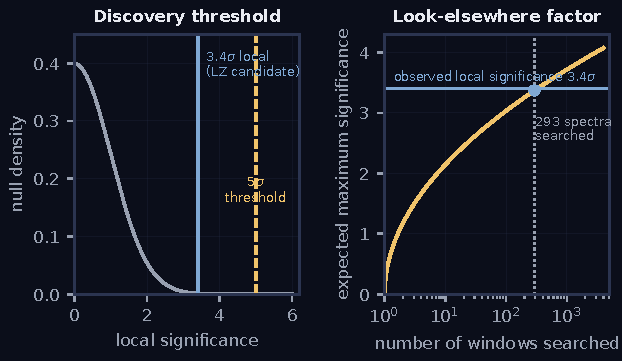
\includegraphics[width=\textwidth]{../figures/fig_event248.pdf}
\caption{The statistical structure of the claim. Left: the null distribution
of the local significance under the Gaussian approximation, with the 5 sigma
discovery threshold and the candidate's local significance. Right: the
expected maximum local significance when $N$ independent windows are
searched, under the same approximation; with 293 spectra the expected maximum
is about 3.4 sigma, which is where the observed value sits.}
\label{fig:event248}
\end{figure}

\section{Why the event is interesting}Three features make it worth attention.

The energy is in the region where a weak-scale WIMP would produce a
recoil, and the implied cross section at that mass is close to the current
exclusion boundary --- which is precisely why the event survived a search
that had already excluded most of the region. It is the first direct-detection
candidate in the field in several years.

The signal is at the high end of the window that LZ's standard analysis
covers, in a region with an extended, higher-energy nuclear-recoil spectrum.
The collaboration had deliberately excluded it from the standard analysis,
which means there is no blinded precedent for the background model in exactly
that window.

Six interpretation papers appeared within four days \idx{LZ 248 keV
interpretations}, which is itself a datum: the field wanted this to be
real.

\section{Why it is not a discovery}The standard for a discovery claim in this
field, adopted across the community and stated explicitly in the recent
discussions of discovery criteria, is at least 5 sigma in at least two
independent experiments with different targets and different systematic
uncertainties \idx{Discovery criteria}. The candidate does not meet it on
either count.

That is not a technicality, and it is worth being precise about why. The
3.4 sigma local significance is computed against a single preselected
window, and the analysis was not blinded: the collaboration had the
opportunity to look at the data and select the window afterwards, and the
global significance of 2.6 sigma is the correction for the fact that many
windows could have been tried. A single event carries no redundancy: there
is no second event, no energy spectrum, no rate consistency check. The
background model in the new window has no blinded validation.

The last point is the one that deserves the most attention, because it is
the failure mode that has produced most of the field's false alarms. The
signal is one event in a window that was chosen with the data in hand. That
is the same structure as the 3.5~keV X-ray line, the 21~cm absorption
anomaly, the EDGES signal, and the Draco dwarf galaxy line --- each of
which was a real measurement, published in good faith, and did not
replicate. Chapter~\ref{ch:indirect} examines that record in detail.

\section{The interpretation papers}The six papers published in the first week fall into
recognisable groups, and their disagreements are informative.

Several treat the event as evidence for a dark matter particle with a
velocity-dependent or energy-dependent interaction, motivated by the
difficulty of reconciling the event with the existing exclusion curves at
the same mass. Others treat it as a constraint on such models, showing that
the required parameter space is small and heavily fine-tuned. Others analyse
the halo model assumptions that the inference depends on, in particular the
local velocity distribution, and show that the inferred cross section is
sensitive to it.

That last group is the most interesting in principle, because it connects
the event to the Solar System programme of Chapter~\ref{ch:solarsystem}. If
the local halo is rotating, or if the dark matter in the Solar System
includes a bound population with a lower velocity, then the velocity
distribution that converts an event into a cross section is not the one
assumed. This is one of the few places where an astrophysical measurement
and a laboratory candidate meet.

\section{What would settle it}Four things would move this candidate, in
increasing order of force.

A \emph{second event} in the same window, from the same data or from more
data, would take the significance up directly and test the background
model. A \emph{reproduction by a different experiment} with a different
target and a different background would be decisive if it exceeded 5 sigma,
and the two-generation suite now under construction is capable of it.
An \emph{exclusion} of the region by an existing experiment that has better
background control in that window would remove the candidate, and this is
not a hypothetical: the window lies above LZ's standard range and other
experiments have different energy reach. A \emph{halo-model measurement} ---
a directional measurement of the local velocity distribution --- would
reduce the interpretive ambiguity without settling the candidate
experimentally.

\section{The honest position}The candidate is worth taking seriously and it is not
a discovery. Both statements are true, and the discipline of holding them
together is the whole content of this chapter. The event is a single
unblinded event at 3.4 sigma local significance in a new window; the field
that has been burned four times in five years by exactly this pattern should
require the standard it has written down, and should require it now rather
than after the next announcement.

\begin{keytakeaways}
\item The observation is one event at 248 keV, 3.4 sigma local and 2.6 sigma
global, in an unblinded analysis of a new energy window, with the data
public.
\item It fails the field's own discovery standard of 5 sigma in two
independent experiments with different targets and systematics.
\item The one-event, unblinded, newly-opened-window structure is the exact
structure of the four anomalies of the last five years that did not
replicate.
\item The dependence of the inferred cross section on the local halo velocity
distribution connects the candidate directly to the Solar System
measurements of Chapter~\ref{ch:solarsystem}.
\end{keytakeaways}
